\chapter{Resultados\label{ch:results}}

% Simple, clear purpose and principles give rise to complex, intelligent behavior. Complex rules and regulations give rise to simple and stupid behavior. (Dee Hock)

% Resumo opcional. Comentar se não usar.
%\resumodocapitulo{Resumo opcional.}

% Resumo informações da arquitetura relevantes do ponto de vista de controle

%\section{Modelagem do Meka}
%\subsection{Estrutura controladores}

% \digraph[scale=0.5]{ab}{rankdir=LR; a->b;}

Para algum conhecimento se tornar cientifico é preciso a sistematização. Nesta capítulo serão apresentados os resultados qualitativos e numéricos do estudo feito em cima da plataforma.

\section{Estudo Arquitetura}

A primeira etapa foi de estudo do código e documentação em busca de identificar tecnologias e algoritmos envolvidos no controle do Meka. O intuito era identificar possíveis referências que ajudasse a guiar os experimentos a serem realizados e eventuais pontos críticos para o desempenho. Como a documentação oficial do Meka foi tirada fora do ar e apenas estão disponíveis as documentações geradas pela comunidade, foi feito um estudo para retirar possíveis pistas através do conhecimento deixado no código dentro do robô. Tal foi somente possível, pois por se tratar de uma plataforma voltada para pesquisa todo o código fonte estava disponível dentro do PC auxiliar.

% Arquitetura comunicação

No que foi 

\begin{figure}
    \centering
    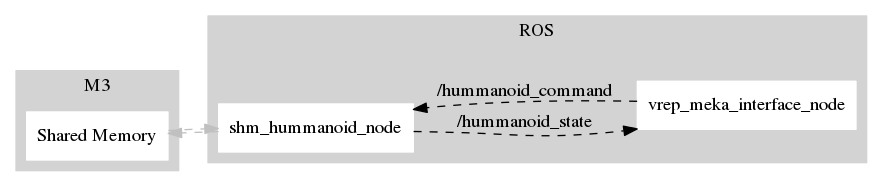
\includegraphics[width=1\linewidth]{figs/shm_arch}
    \caption{Caption}
    \label{fig:my_label}
\end{figure}


Todo o código relacionado ao controle do robô é disponibilizado pelo fabricante e compõe a biblioteca M3, implementada em Python e com interface em C++. A partir da análise do código foi possível observar alguns pontos importantes que contribuem para ineficiência dos controladores implementado anteriormente:

\begin{itemize}
    \item Apenas controle por posição de juntas está implementado em C++
    \item A taxa de atualização da memória compartilhada é de $100 Hz$
\end{itemize}

Dentro do programa de interface com o ROS foi possível observar alguns pontos importantes que contribuem para ineficiência dos controladores controladores de posição com e sem compensação da gravidade. Os valores de velocidade e torque informados para o controle são completamente ignorados. Além disto a taxa de envio da informação obtida pelo ROS para a memória compartilhada é de apenas $100Hz$ definidos \textit{hardcode}. Foi feito um teste para alterar este valor para $1KHz$ porém o robô ficou completamente instável. De movo que novos testes não foram repetidos para evitar danos ao robô.

Este valor é bem próximo das taxas de amostragem de $8 ms$ ($125 hz$) e $20 ms$ ($50 Hz$) dos controladores implementados em C++ obtidas para os melhores resultados em \cite{nobody} obtidos por Marco Pereira. Sendo estes valores definidos pelo tempo mínimo necessário para efetuar todos os cálculos relacionados ao controladores cinemáticos implementados usando quatérnions duais.

\section{Estudo Controladores Meka}

\subsection{API Python}

Para avaliar os controladores de junta de baixo nível foi utilizado a API em Python e a partir dai foram feitos vários teste a partir de comandos de posição para as juntas. A estrutura para envio dos comandos para o robô é diferente, de modo que alguns testes relacionados a comunicação também foram necessários. Estão estão disponíveis os seguintes controladores, ordenados do de mais alto nível para o de mais baixo nível:

\begin{itemize}
    \item Posição
    \item Velocidade
    \item Torque
    \item PWM
\end{itemize}

Todos estes estão disponíveis nos modos com e sem compensação da gravidade. 

\subsubsection{Avaliação do Atraso de Comunicação}

A comunicação com o robô é feita através de uma memória compartilhada. Assim, o primeiro experimento foi levantar o tempo gasto pela instrução \textit{proxy.step()} que atualiza esta memória pegando as medidas dos sensores e informando os comandos para os controladores. Este teste foi feito através avaliando o intervalo de tempo entre cada chamada após sucessivas interações tendo como resultado o valor médio de 16ms entre cada chamada indicando que a frequência máxima possível para um controlador implementado com base na API é de $f = 1/16ms = 62.5Hz$. Isto, obviamente, desconsiderando qualquer tempo extra gasto com as operações realizadas pelo próprio controlador.

\subsubsection{Avaliação do Acumulo do Erro}

Para verificar o acumulo do erro após sucessivas interações foi feito o teste de fechar a malha com braço na posição de repouso. Isto é, controle deveria ler os dados atuais do sensores e passar diretamente para o robô na expectativa de que o robô ficasse parado. No entanto foi observado que o braço começou a subir lentamente, indicando valores cada vez maiores para os ângulos medidos e uma distância cada vez maior da posição de origem.

Por outro ao ser enviado a mesma posição de referência suscetivamente, o braço desloca até o ponto desejado e permanece parado, mostrando que o controle para um referência em degrau é estável. O que viabilizou os testes de identificação a partir do uso de uma entrada em Degrau.

\subsubsection{Entrada em rampa}

Foram então feitos testes para um referência em rampa. Como se trata de um controle feito de maneira discreta, foram passados valores de ângulos em sequência incrementados por um valor contante e separados por um pequeno tempo de espera emulando uma entrada em rampa porém discretizada no tempo.

Para estudo da velocidade de resposta do controlador, o valor incrementado entre um ângulo e outro foi mantido enquanto o intervalo de tempo era ajustado. Neste experimento foi observado que para intervalos muito pequenos de tempo o robô não consegue acompanhar mantendo uma velocidade constante. Em tais casos a velocidade é mantida aproximadamente constante e com o acúmulo do erro ocorre saltos periódicos para compensar o atraso em relação a referência. Este fato decorre da interação entre o controlador de posição das juntas e o controlador de torque. O erro acumulado é corrigido com a passagem de um torque mais alto produzindo um salto na posição, seguido de uma leve oscilação para compensar o efeito da inercia.

% Repete testes ?

\subsubsection{Resposta ao Degrau}

Feito uma avaliação preliminar para o experimento de identificação da planta foi aplicado um degrau para cada uma das juntas individualmente com registro dos dados. Este teste foi definido a partir dos seguintes passos:

\begin{enumerate}
    \item Começa com a junta na posição $0$ graus
    \item Envia o comando para ir para posição $45$ graus
    \item Mantém a referência da posição em $45$ graus por $2s$
    \item Envia o comando para ir para posição $0$ graus
    \item Mantém a referência da posição em $0$ graus por $2s$
\end{enumerate}

Para a API em Python Estes passos foram executados 3 vezes para cada uma das juntas. O mesmo experimento foi efetuado a partir de um programa em C++ baseado no código elaborado em trabalhos anteriores. Para ambos casos a saída dos sensores foi registrada a partir do ROS a partir do programa rosbag e somente para os testes feitos em C++ foram também registradas os mensagens de controle. Uma vez que os comandos passados via API são enviados diretamente para o serializador de mensagens sem passar pelo ROS e portanto foram utilizados apenas para uma avaliação preliminar do comportamento dos controladores de junta.

% Qual foi a diferença dos dois para os mesmo parâmetros?
% Por que não foram avaliados outros ângulos?

\subsubsection{Controle de Posição sem Compensação da Gravidade}

O controle de posição sem o uso de compensação da gravidade foi avaliado em estudo e não foi possível atingir a posição desejada de 45 graus partido do zero em nenhuma das juntas. Na maioria dos caso o braço movia apenas 10 graus. O que explicita que toda a estratégia de compensação da gravidade é feita por software, diferente de outras plataformas como o Baxter em que esta é feita de forma mecânica.

\subsubsection{Controle de Velocidade}

Foi feito apenas um ensaio utilizando o controle de velocidade disponível na API em Python. No entanto ao ser definido velocidade zero a braço robótico ficou completamente rígido e passou a ignorar comandos para outros valores de referência de velocidade. O que demonstrou um esforço grande sendo feito pelo controle de torque e pelos motores. Somente quando foi alterado o modo de controle para posição que o braço voltou a mover normalmente. Para evitar qualquer dano a plataforma, não foram feitos outros testes neste modo de operação.

% Teria como controlar a velocidade diretamente ?

\subsubsection{Controle de Torque}

O controle de torque está disponível em dois modos: com e sem compensação da gravidade. Na estratégia sem compensação da gravidade, o valor de referência de torque é passado diretamente a controlador das juntas.

% Por que não foi avaliado o controle de torque?

\section{Estudo Controladores Cinemáticos}

\subsection{Resposta ao Degrau C++}

A velocidade máxima de cada junta pode ser ajusta para um valor entre $0$ e $1$, de igual forma a rigidez do braço gerada pelo controlador também pode ser ajustada entre $0$ e $1$. Valores maiores que 1 foram testados porém não houve mudança significativa em relação a comportamento com valor $1$.

Já no experimento feito de referência mostrado na \ref{fig:jointIdentification_exp2v100v50}, pode-se notar que existe um atraso de cerca de $20ms$ entre o comando e o recebimento do sinal de resposta do atuador no tópico. Também percebe-se um erro grande em regime permanente das juntas do pulso ($5$ e $6$). Percebe-se uma longa rampa indicando aonde o controle da posição passou a atuar como um controle tudo ou nada passando a velocidade máxima possível. Curiosamente, embora sejam motores distintos em cada uma das juntas com diferentes limites de velocidade a resposta do controlador é indica uma velocidade bem parecida de atuação nesta configuração.

\begin{figure}[H]
    \centering
    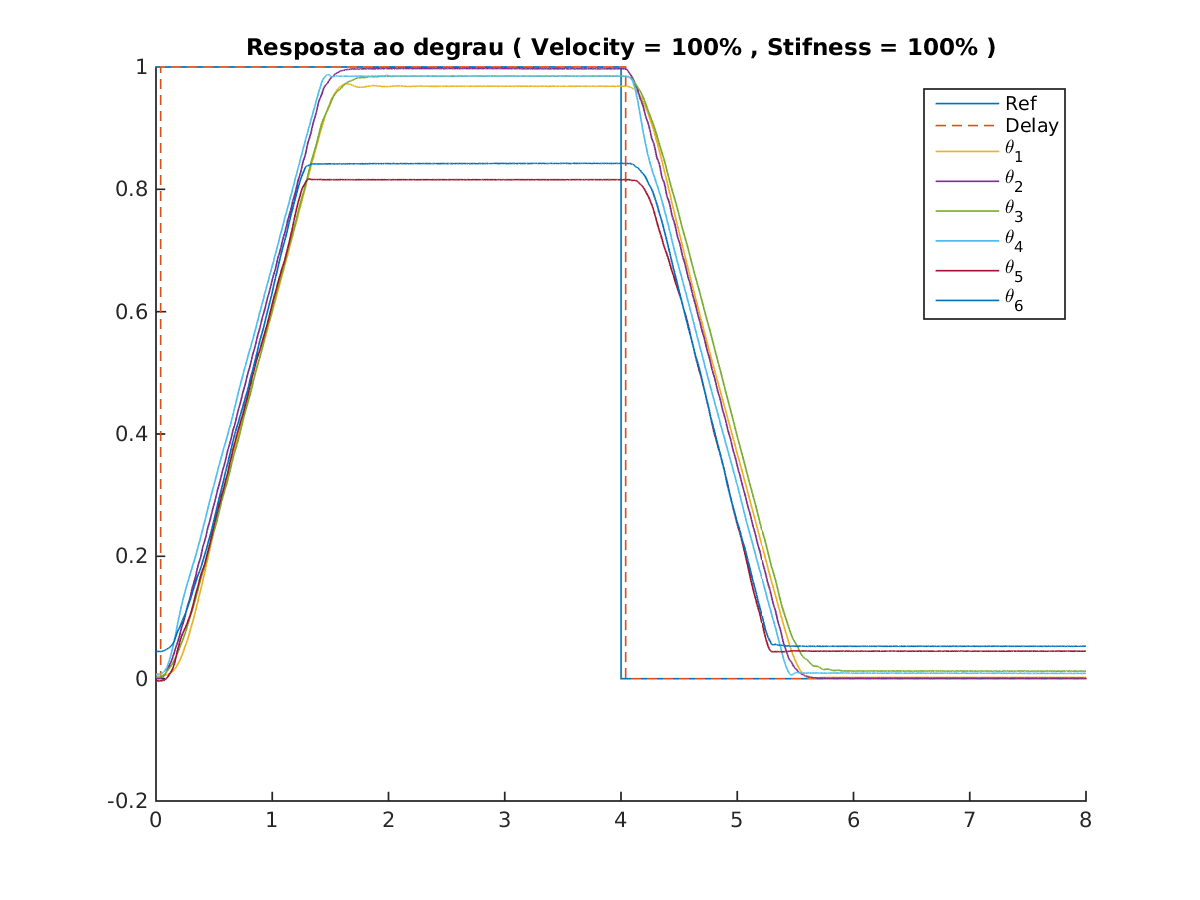
\includegraphics[width=0.6\linewidth]{tex/figs/jointIdentification_exp1v100v100.png}
    \caption{Resposta a um degrau de entrada com Velocidade = 1 e Rigidez = 1}
    \label{fig:jointIdentification_exp1v100v100}
\end{figure}

Pela figura \ref{fig:jointIdentification_exp2v100v50} observa-se que a variação da rigidez do controlador implica em um erro maior em regime permanente nas juntas. O controlador converge em um tempo próximo mas notadamente aumenta o erro das juntas do pulso. Este fato também é percebido no código de demonstração no ajuste da rigidez. Pois ao mudar o valor, mantida a mesma referência de posição o pulso desloca significativamente de posição.

\begin{figure}[H]
    \centering
    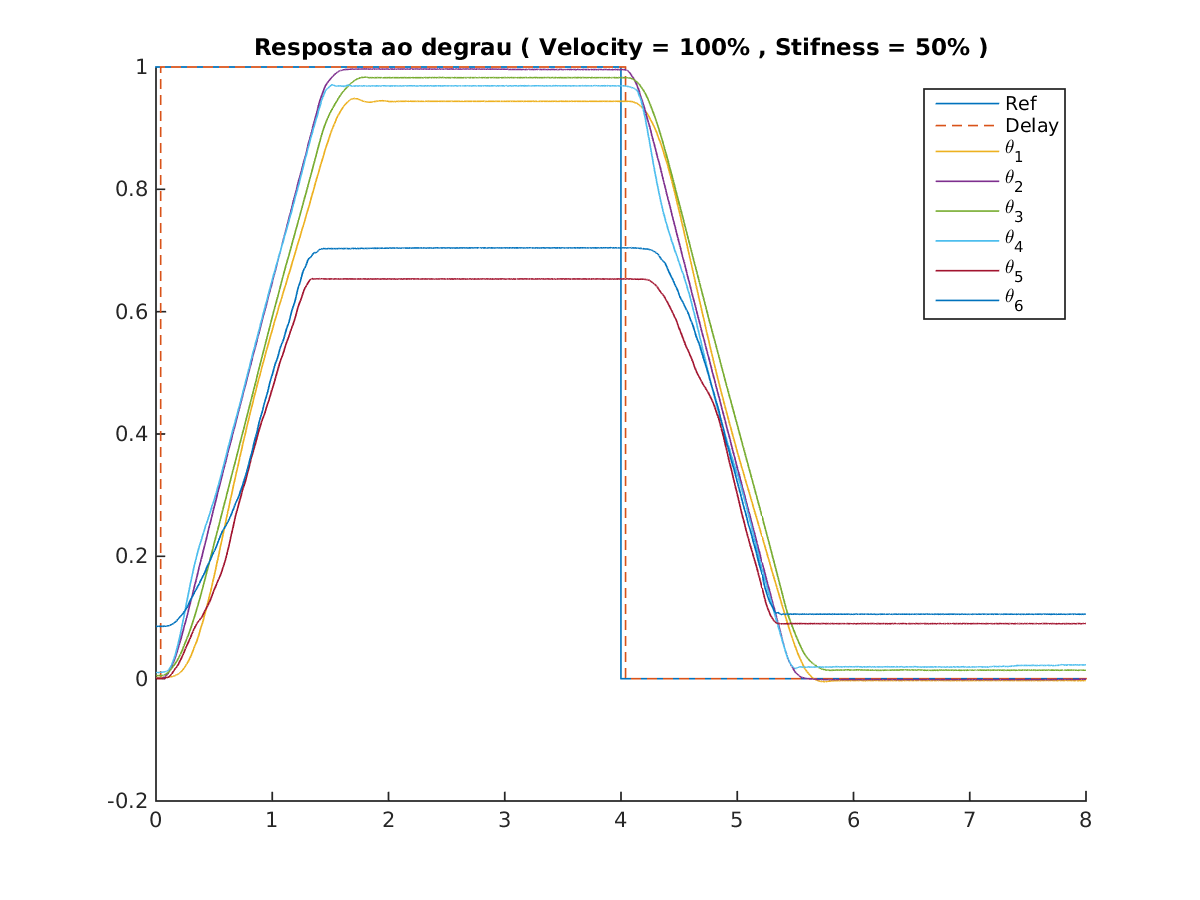
\includegraphics[width=0.6\linewidth]{tex/figs/jointIdentification_exp2v100v50.png}
    \caption{Resposta a um degrau de entrada com Velocidade = 1 e Rigidez = 0.5}
    \label{fig:jointIdentification_exp2v100v50}
\end{figure}

Como esperado, no terceiro experimento ao se alterar a velocidade para $70\%$ o tempo necessário para cada uma das juntas atingir a posição aumentou, tendo em vista a fase em que o controlador utiliza a velocidade máxima permitida, o erro em regime permanente para cada um permanece com pouca alteração. No entanto é percebido que a inclinação da curva durante as fase de controle entre o tempo $t=1s$ e $2s$ com a velocidade máxima muda de forma diferente para cada uma duas juntas. Estes dados encontram-se na figura \ref{fig:jointIdentification_exp3v70v100}.

\begin{figure}[H]
    \centering
    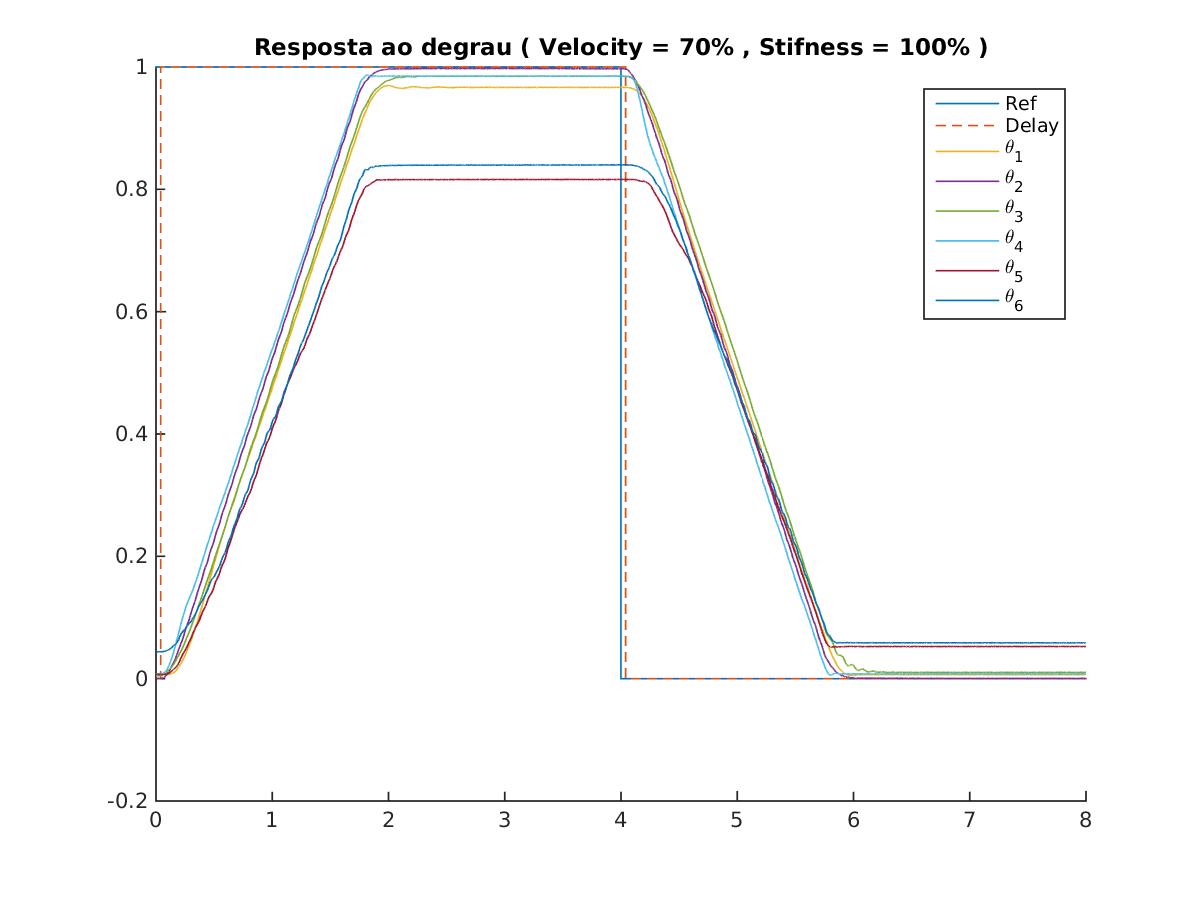
\includegraphics[width=0.6\linewidth]{tex/figs/jointIdentification_exp3v70v100.png}
    \caption{Resposta a um degrau de entrada com Velocidade = 0.7 e Rigidez = 1}
    \label{fig:jointIdentification_exp3v70v100}
\end{figure}

No 3 experimentos o atraso obtido foi próximo de $20ms$. Este valor é próximo dos valores de intervalo de tempo obtidos para os melhores resultados dos controladores implementados em \ref{nocite}. Notadamente, quando o controlador opera com frequências maiores, haverá o impacto do atraso da comunicação passa a ser mais significativo levando a instabilidade caso este não seja considerado no dinâmica implementada.


Tomando-se o diferença entre o valor passado de referência e o valor alcançado tempo foram obtidos os erro em regime permanente, registrados na tabela \ref{tab:jointIdentification_errortable}.

\begin{table}[H]
    \centering
    $$\begin{array}{cc|ccccccc}
         \hline
         V & S & \theta_0 & \theta_1 & \theta_2 & \theta_3 & \theta_4 & \theta_5 & \theta_6\\
         \hline
         -Inf & 0.031544 & 0.0025193 & 0.014824 & 0.014865 & 0.18436 & 0.15769\\
-Inf & 0.056071 & 0.0036188 & 0.017413 & 0.031003 & 0.34662 & 0.29566\\
-Inf & 0.033305 & 0.0026167 & 0.015199 & 0.014783 & 0.18398 & 0.16037\\
-Inf & 0.056453 & 0.0035564 & 0.017352 & 0.03028 & 0.32879 & 0.28538\\

         \hline
    \end{array}$$
    \caption{Error Percentual para diferentes valores de velocidade ($V$) e rigidez ($S$)}
    \label{tab:jointIdentification_errortable}
\end{table}

\begin{table}[H]
    \centering
    $$\begin{array}{cc|ccccccc}
         \hline
         V & S & \theta_0 & \theta_1 & \theta_2 & \theta_3 & \theta_4 & \theta_5 & \theta_6\\
         \hline
         0 & 1.0041 & 1.0001 & 1.0002 & 1.0025 & 1.0016 & 0\\
0 & 1.0049 & 1.0004 & 1.0008 & 1.0019 & 1.0007 & 0\\
0 & 1.003 & 1.0002 & 1.0004 & 1.0016 & 0 & 0\\
0 & 1.005 & 1.0004 & 1.0009 & 1.0026 & 0 & 0\\

         \hline
    \end{array}$$
    \caption{Percentual Overshot para diferentes valores de velocidade ($V$) e rigidez ($S$)}
    \label{tab:jointIdentification_overshottable}
\end{table}

\begin{table}[H]
    \centering
    $$\begin{array}{cc|ccccccc}
         \hline
         V & S & \theta_0 & \theta_1 & \theta_2 & \theta_3 & \theta_4 & \theta_5 & \theta_6\\
         \hline
         1.00 & 1.00 & 0.001841 & 0.96846 & 0.99748 & 0.98518 & 0.98513 & 0.81564 & 0.84231\\
1.00 & 0.50 & 0.003698 & 0.94393 & 0.99638 & 0.98259 & 0.969 & 0.65338 & 0.70434\\
0.70 & 1.00 & 0.0020654 & 0.9667 & 0.99738 & 0.9848 & 0.98522 & 0.81602 & 0.83963\\
1.00 & 0.50 & 0.0047216 & 0.94355 & 0.99644 & 0.98265 & 0.96972 & 0.67121 & 0.71462\\

         \hline
    \end{array}$$
    \caption{Valor em regime permanente para diferentes valores de velocidade ($V$) e rigidez ($S$)}
    \label{tab:jointIdentification_steadstatetable}
\end{table}

\subsection{Controladores Cinemáticos usando Quatérnions Duais}

% Experimento MoveUP

Os controladores de posição do efetuador foram avaliado a partir da estratégia de discretização dos pontos e frequência de amostragem. Para tal foi reduzido o número de ponto e trajetória foi simplificada para apenas um deslocamento em linha reta de 10cm na vertical. Para primeira análise foi utilizado os controladores implementados anteriormente e foram feitos os seguintes testes:

\begin{enumerate}
    \item Trajetória dividida em $100$ pontos, intervalo de $8 ms$
    \item Trajetória dividida em $100$ pontos, intervalo de $100 ms$
    \item Trajetória dividida em $1000$ pontos, intervalo de $8 ms$
\end{enumerate}

Foi observado que o robô leva um tempo até começar a mexer e um tempo até o controle estabilizar. De modo que está sempre atrasado em relação a referência. Para o período $8 ms$ foram necessárias $25$ interações até o robô começar a se mover, com o período de $100 ms$ o robô começo a se mover já na segunda interação sugerindo um atraso na comunicação de $200 ms$ entre o tempo que o comando é passado via ROS e o tempo que o robô executa o comando.

% Gráficos ?

% Saltos a cada 300 ms

\section{Estudo sobre não linearidades}

% Acrescentar simulação no simulink pControlSaturation
% - Comparativo da resposta para o mesmo ganho em um sistema de primeira ordem ( com delay e saturação )
% - Verificar necessidade de mudar a ordem e puxar a seção para antes

Uma vez que os modelos usados para o controle são lineares, a existência de comportamentos não lineares representam perturbações e podem gerar erros ou até instabilidade no controle caso não consideradas. Em razão disto uma atenção especial foi dada a este aspecto visando identificar a contribuição da perca de desempenho. A grande dificuldade é podem ocorrem em qualquer uma das partes do sistema de controle gerando um acumulo do efeito com o aumento da quantidade de camadas em cascata.

\subsection{Saturação do Atuador}

O efeito de saturação do atuador ocorre quando é solicitado uma ação de torque ou velocidade acima do que o atuador permite. Em diversos sistemas isto é limitado através de algum dispositivo de proteção evitando danificar o atuador. Do lado do controle, este é percebido como uma resposta mais lenta que o esperado para aquele determinado ganho em simulação podendo levar a instabilidade no controle do sistema real.

Como o controle da posição é feito em colaboração pela ação de cada uma das juntas, este problema é mascarado na métrica do erro de posição. Como a contribuição de cada junta em manipulador não cartesiano muda de acordo com a posição, o atraso devido a saturação pode fazer com que o robô tenha um erro maior para determinadas posições no decorrer da trajetória que outras. Outro efeito é a saturação de um motor levar a um uso maior dos outro motores na tentativa de compensar o erro acumulado.

São utilizados diferentes motores para cada uma das juntas, conferindo limitações especificas na atuação, em particular na velocidades máximas que cada junta pode atingir. Por conta disto, é percebido um maior uso das juntas com velocidade máxima maior para compensar o erro acumulado pela juntas com velocidade máxima menor, quando o controle começa solicitar uma velocidade maior que a permitida pelos outros motores.

Em particular no Meka, este fenômeno leva a um uso maior das juntas do ombro para corrigir orientação ao invés das juntas do pulso. Sendo um braço antropomórfico, o comportamento intuitivo esperado é a preferência das juntas mais próximas ao tronco para atuarem mais na posição enquanto as juntas próximos ao efetuador corrigirem a orientação. Isto é refletido na Jacobiana, para uma mesma variação de ângulo o mudança na posição e orientação é maior para as juntas do ombro que para as juntas do pulso.

% Fenômeno Harakiri: O cotovelo do meka vai se aproximando do tronco com o passar do tempo, o robô move bruscamente com pertubações na orientação a partir da posição de referência usada nos trabalhos do Koji e do Marcos

% Montar experimento Harakiri 2DOF
% Montar experimento Harakiri Meka em simulação no Matlab
% Montar experimento Harakiri Meka real
% Estudo do erro por junta ao invés de por posição -> Pontuar necessidade introduzir novas métricas

\subsection{Atraso da Comunicação}

Dado a existência de várias camadas entre o controle cinemático e o atuador de fato, existe um atraso na comunicação que influência na dinâmica do sistema. O controlador cinemático interagem com o ROS que por sua vez interage com uma memória compartilhada que é atualizada com um frequência de $1 KHz$. Para avalia o atraso foi feito a medida a partir do ensaio em degrau, entre o tempo de envio do comando de controle no tópico $/humanoid_control$ e o primeiro instante em que a posição da junta atinge um valor diferente de zero na leitura do valor correspondente no tópico $/humanoid_state$. Uma vez que existe um pouco de ruído na leitura da posição, foi considerado a valor de referência $\Delta\theta_0 = 0.1 rad = 5^\circ$.

% Resultados

\subsection{Controle Virtual de Rigidez}

% Comparar com primeiras implementações de SEA

Com base no controle do torque e o uso de sensores de posição pode se emular o comportamento de uma mola com rigidez variável através de um controlador. Esta estratégia é denominada mola virtual e permite conferir o controle de força com precisão sem a necessidade de ajustar fisicamente algum elemento elástico.

% Diagrama SEA Virtual